\providecommand{\isolatedBuild}[1]{#1}% fallback definition lets this file build normally
\isolatedBuild
{
\documentclass[11pt,letterpaper]{book}
\usepackage{import}

% This file must be found via the TEXINPUTS environment variable.
%\documentclass[11pt,letterpaper]{book}

% aleeper: I think these are needed for Paul's macros?
\usepackage{epsfig}
\usepackage{epstopdf}

%\makeatletter
%\typeout{The import path is \import@path}
%\makeatother

\usepackage{import}

\subimport{./}{packagesMitiguy.sty}
\subimport{./}{macrosMitiguy.tex}
\subimport{./}{PageStylesMitiguy.tex}
\subimport{./}{macrosLeeper.tex}


\pagestyle{empty}
\pagenumbering{arabic}

\begin{document}
\HandoutHeader{Vector Equations and Geometry}
\normalsize
\vspace{-1.5pc}
\\[0.0pc]
%
%\begin{enumerate}
%\item
\textColorBold{darkerBlue}{Polygon Meshes in Engineering and Graphics}
\\[0.5pc]
}
%%%%%%%%%%%%%%%%%%%%%%%%%%%%%%%%%%%%%%%%%%%%%%%%%%%%%%%%%%%
%
%
\begin{minipage}[t]{0.68\columnwidth}
In many engineering applications (such as stress and aerodynamics computations using finite elements, as well as CAD and graphical display), objects are represented using a group of polygons. Being able to compute a ``normal'' vector perpendicular to each polygon is important for all these applications.
\end{minipage}
\hfill
\begin{minipage}[t]{0.25\columnwidth}
\flushright
\vspace*{0pc}
%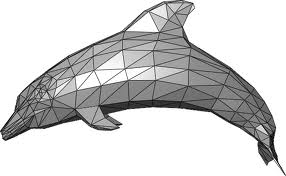
\includegraphics[width=0.95\columnwidth]{dolphin.jpg}
%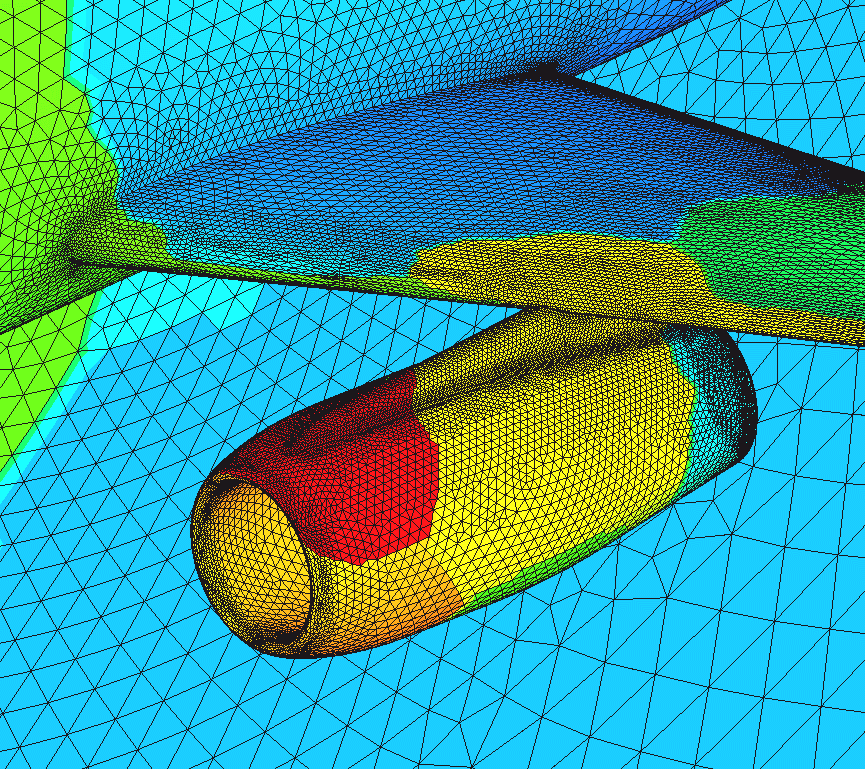
\includegraphics[width=0.9\columnwidth]{wing_mesh.png}
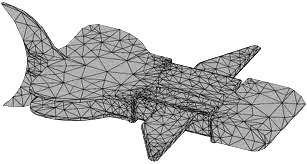
\includegraphics[width=0.97\columnwidth]{wing_robot.jpg}
\end{minipage}
%\\[0.0pc]
%For example, for drawing a polygon on screen, it is necessary to compute the illumination in a way that simulates realistic lighting. A simple model for diffuse illumination at each vertex (corner) of a polygon is defined as $I_D = I_L * \uvecWithHat{n} \cdot \uvecWithHat{L}$, where:
%\begin{itemize}
%\item $I_L$ is the (scalar) strength of the incoming light.
%\item $\uvecWithHat{L}$ is the unit vector from the vertex to the light source.
%\item $\uvecWithHat{n}$ is the ``unit-normal" for the polygon (that is, the unit vector perpendicular to the polygon).
%\end{itemize}
%
\\[0.5pc]
In the figure below, the \uvecxyz{a} ``coordinate" measures of each vertex from $A_o$ are labeled.
\\[0.0pc]
For example, $\posvec{A_o}{P_1} \equals[\;] 3~\uvecx{a} \plus[\;] 2~\uvecy{a} \plus[\;] 0~\uvecz{a}$.
\begin{enumerate}
\item \underline{Compute} a vector \bvec{n} that is perpendicular to the polygon, expressed in \uvecxyz{a}.
\item \underline{Explain} in detail how to get \uvecWithHat{n}, the unit vector in the same direction as \bvec{n}. \underline{Sketch} \uvecWithHat{n} on the figure.
\item \underline{Explain} why there are actually two possible \uvecWithHat{n} vectors for the polygon.
%\item Compute \posvec{P_0}{Q}, and hence compute the unit vector $\uvecWithHat{L}$.
%\item For a light source of strength $I_L = 0.5$, compute the diffuse illumination $I_D$.
\end{enumerate}
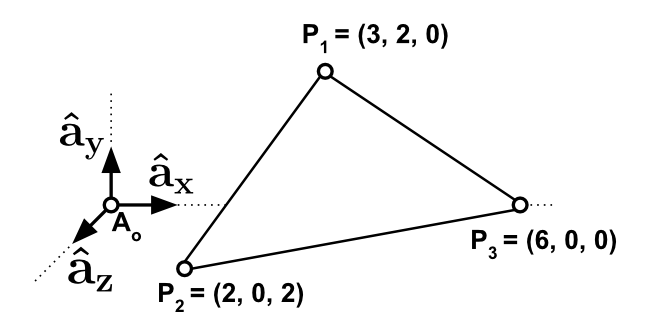
\includegraphics[width=8cm]{polygon_normal.png}

\vfill
Bonus (1 pt). What is the geometric interpretation of the length of \bvec{n}?
\vspace{2.0pc}

\isolatedBuild {
%\end{enumerate}
 \end{document} }
